% This file includes the formatting guidelines for papers submitted to 'Inteligencia Artificial' (Revista Iberoamericana de IA)
% It should be used jointly with file iberamia.sty

\documentclass[10pt,a4paper,twoside]{article}
\usepackage[english]{babel}
\usepackage[latin1]{inputenc}
\usepackage{amssymb}
\usepackage{amsmath}
\usepackage{fancyhdr}
%\usepackage[usenames,dvips]{color}
\usepackage{verbatim}
\usepackage{lastpage}
\usepackage{ifthen}
\usepackage{csquotes}
\usepackage{cite}
\usepackage{listings}
\newcommand{\norm}[1]{\left\lVert#1\right\rVert}
\DeclareMathOperator*{\argmin}{arg\,min}
\DeclareMathOperator*{\argmax}{arg\,max}


%%%%%%%%%%%%%%%%%%%%%%%%%%%%%%%%%%%%%%%%%%
%                                        %
% IMPORTANT FOR USERS OF PDFLATEX        %
%                                        %
%%%%%%%%%%%%%%%%%%%%%%%%%%%%%%%%%%%%%%%%%%
%
% We assume LaTeX users will use PDFLaTeX
% Comment the next lines if you wish to use dvipdfm instead.
\usepackage[pdftex]{color,graphicx}
\usepackage{hyperref}
%
% Remove comment if you wish to use dvipdfm to generate PDF files.
%\usepackage{epsfig}
%\usepackage[dvipdfm]{hyperref}
%
%%%%%%%%%%%%%%%%%%%%%%%%%%%%%%%%%%%%%%%%%%

\usepackage{iberamia}   %Journal's style file iberamia.sty

%Publication data:
\newcommand{\thispaperdoi}{}
\setcounter{year}{2017}
\setcounter{volume}{20}
\setcounter{issue}{59}
\setcounter{page}{123}

\lstset{
  backgroundcolor=\color[rgb]{0.9,0.9,0.9},
  tabsize=4,
  language=C++,
  captionpos=b,
  tabsize=3,
  frame=lines,
  numbers=left,
  numberstyle=\tiny,
  numbersep=5pt,
  breaklines=true,
  showstringspaces=false,
  basicstyle=\footnotesize,
  identifierstyle=\color{magenta},
  keywordstyle=\color[rgb]{0,0,1},
  commentstyle=\color[rgb]{0.026,0.112,0.095},
  stringstyle=\color{red},
  }

\title{From Imitation to Prediction, Data Compression vs Recurrent Neural Networks for Natural Language Processing}

%%NOTE: If you are submitting for review, do not include author's data
%       The journal uses a double-blind review processe

\author{Juan Andr�s Laura, Gabriel Omar Masi, Luis Argerich
\smallskip \\
\small{Departemento de Computaci�n,
	Facultad de Ingenier�a. Universidad de Buenos Aires
\smallskip \\
jandreslaura@gmail.com, masigabriel@gmail.com, largerich@fi.uba.ar 
}}
\date{}

\begin{document}

\medskip
\maketitle

\pagestyle{Rest}
\thispagestyle{FirstPage}
\smallskip


\noindent{\small{{\textbf Abstract}
In recent studies \cite{Graves}\cite{Sutskever}\cite{Bown} Recurrent Neural Networks were used for generative processes and their surprising performance can be explained by their ability to create good predictions. In addition, data compression is also based on prediction. What the problem comes down to is whether a data compressor could be used to perform as well as recurrent neural networks in the natural language processing tasks of sentiment analysis and automatic text generation. If this is possible, then the problem comes down to determining if a compression algorithm is even more intelligent than a neural network in such tasks. In our journey, a fundamental difference between a Data Compression Algorithm and a Recurrent Neural Network has been discovered. }}


\medskip

\noindent{\small{\textbf{Keywords}: Natural language processing, Compression algorithms, Neural networks, Predictions.}}


\section{Introduction}
One of the most interesting goals of Artificial Intelligence is the simulation of different human creative processes like speech recognition, sentiment analysis, image recognition, automatic text generation, etc. In order to achieve such goals, a program should be able to create a model that reflects how humans think about these problems.

Researchers think that Recurrent Neural Networks (RNN) are capable of understanding the way some tasks are done such as music composition, writing of texts, etc. Moreover, RNNs can be trained for sequence generation by processing real data sequences one step at a time and predicting what comes next\cite{Graves}\cite{Sutskever}.

Compression algorithms are also capable of understanding and representing different sequences and that is why the compression of a string could be achieved. However, a compression algorithm might be used not only to compress a string but also to do non-conventional tasks in the same way as neural nets (e.g. a compression algorithm could be used for clustering\cite{Cilibrasi}, sequence generation or music composition).

Both neural networks and data compressors should be able to learn from the input data to do the tasks for which they are designed. In this way, someone could argue that a data compressor can be used to generate sequences or a neural network can be used to compress data. In consequence, using the best data compressor to generate sequences should produce better results than the ones obtained by a neural network but if this is not true then the neural network should compress better than the state of the art in data compression.

The hypothesis for this research is that, if compression is based on learning from the input data set, then the best compressor for a given data set should be able to compete with other algorithms in natural language processing tasks. In the present work, this hypothesis will be analyzed for two given scenarios: sentiment analysis and automatic text generation.

\section{RNNs for Data Compression}

Recurrent Neural Networks and in particular LSTMs were used not only for predictive tasks\cite{Gers} but also for Data Compression\cite{Schmidhuber}. While the LSTMs were brilliant in their text\cite{Sutskever}, music\cite{Bown} and image generation\cite{Gregor} tasks, they were never able to defeat the state of the art algorithms in Data Compression\cite{Schmidhuber}. 

This might indicate that there is a fundamental difference between Data Compression and Generative Processes and between Data Compression Algorithms and Recurrent Neural Networs. After experiments, a fundamental difference will be shown in this research in order to explain why a RNN can be the state of the art in some generatives process but not in Data Compression.

\section{Data Compression as an Artificial Intelligence Field}

For many authors there is a very strong relationship between Data Compression and Artificial Intelligence\cite{Franz}\cite{Ofir}. Data Compression is about making good predictions \cite{Ratsaby} which is also the goal of Machine Learning, a field of Artificial Intelligence. 

Essentially, Data compression involves two important steps: modeling and coding. Coding is a solved problem using arithmetic compression. The difficult task is modeling because it comes down to building a description of the data using the most compact representation; this is again directly related to Artificial Intelligence. Using the Minimal Description Length principle\cite{Grunwald} the efficiency of a good Machine Learning algorithm can be measured in terms of how good it is to compress the training data plus the size of the model itself.

A file containing the digits of $\pi$ can be compressed with a very short program able to generate those digits, gigabytes of information can be compressed into a few thousand bytes. However, the problem arises when trying to find a program capable of understanding that our input file contains the digits of $\pi$. In consequence, achieving the best compression rate involves finding a program able to always find the most compact model to represent the data and that is clearly an indication of intelligence, perhaps even of General Artificial Intelligence. 

\section{Sentiment Analysis}

\subsection{A Qualitative Approach}

Human feelings can be determined according to what they write in many social networks such as Facebook, Twitter, etc.. It looks like an easy task for humans. However, it could be not so easy for a computer to automatically determine the sentiment behind a piece of writing.

The task of guessing the sentiment of text using a computer is known as Sentiment Analysis and one of the most popular approaches for this task is to use neural networks. In fact, Stanford University created a powerful neural network for sentiment analysis\cite{Socher} which is used to predict the sentiment of movie reviews taking into account not only the words in isolation but also the order in which they appear. In the first experiment, the Stanford neural network and a PAQ compressor\footnote{PAQ's source code is free and it is available at Mahoney's web \cite{Mahoney}}\cite{Mahoney} will be used for doing sentiment analysis of movie reviews in order to determine whether a user likes or not a given movie (i.e. each movie review will be classified as positive or negative). After that, results obtained will be compared using the percentage of correctly classified movie reviews. Both algorithms will use a public data set for movie reviews\cite{Maas}.

In order to understand how sentiment analysis could be done with a data compressor it is important to comprehend the concept of using Data Compression to compute the distance between two strings using the \textit{Normalized Compression Distance}\cite{Vitanyi}.

$$
NCD(x,y) = \frac{C(xy)-\min\{C(x),C(y)\}}{\max\{C(x),C(y)\}}
$$

Where $C(x)$ is the size of applying the best possible compressor to $x$ and $C(xy)$ is the size of applying the best possible compressor to the concatenation of $x$ and $y$. 

The NCD is an approximation to the Kolmogorov distance between two strings using a Compression Algorithm to approximate the complexity of a string because the Kolmogorov Complexity is uncomputable. 

The principle behind the NCD is quite simple: when string $y$ is concatenated after string $x$ then $y$ should be highly compressed whenever $y$ is very similar to $x$ because the information in $x$ contains everything needed to describe $y$. An observation is that $C(xx)$ should be equal, with minimal overhead difference to $C(x)$ because Kolmogorov complexity of a string concatenated to itself is equal to the Kolmogorov complexity of the string. 

As introduced, a data compressor performs well when it is capable of understanding the data set that will be compressed. This understanding often grows when the data set becomes bigger and in consequence compression rate improves. However, it is not true when future data (i.e. data that has not been compressed yet) has no relation with already compressed data because the more similar the information it is the better compression rate is achieved. 

Let $C(X_1,X_2...X_n)$ be a compression algorithm that compresses a set of n files denoted by $X_1,X_2...X_n$. Let $P_1,P_2...P_n$ and $N_1,N_2...N_m$ be a set of $n$ positive reviews and $m$ negative reviews respectively. Then, a review $R$ can be predicted positive or negative using the following inequality:

$$C(P_1,...P_n,R)-C(P_1,...,P_n) < C(N_1,...,N_m,R)-C(N_1,...,N_m)$$

The formula is a direct derivation from the NCD. When the inequality is not true, a review is predicted negative. 

The order in which files are compressed must be considered. As you could see from the proposed formula, the review $R$ is compressed last. 

Some people may ask why this inequality works to predict whether a review is positive or negative. So it is important to understand this inequality. Suppose that the review $R$ is a positive one. $R$ will be compressed in order to classify it: if $R$ is compressed after a set of positive reviews then the compression rate should be better than the one obtained if $R$ is compressed after a set of negative reviews because the review $R$ has more related information with the set of positive reviews and in consequence should be compressed better. Interestingly, both the positive and negative set could have different sizes and that is why it is important to subtract the compressed file size of both sets in the inequality. Consider the following example:

\begin{displayquote}
\textit{My favorite movie. What a great story this really was. I'd just like to be able to buy a copy of it but this does not seem possible.}
\end{displayquote}

The previous review has a size of 132 bytes. After compressing the train dataset, the results are:

\begin{displayquote}
$C(P_1,...,P_n,R)-C(P_1,...,P_n)$: 42 bytes\\
$C(N_1,...,N_n,R)-C(N_1,...,N_n)$: 43 bytes
\end{displayquote}

Given the previous results, the review $R$ is predicted positive because $C(P_1,...,P_n,R)-C(P_1,...,P_n)$ is lower than $C(N_1,...,N_n,R)-C(N_1,...,N_n)$.


\subsection{PAQ for Sentiment Analysis}

Using Data Compression for Sentiment Analysis is not a new idea. It has been already proposed in IEEE 12th International Conference\cite{Ziegelmayer}. However, the authors did not use PAQ compressor.

PAQ Compressor is taken into account for this research because of its excellent compression rates achieved at Hutter's Prize\cite{Hutter} and many benchmarks such as Matt Mahoney's one\cite{Mahoney}.

In order to make sentiment analysis of a movie review using PAQ, it is needed to compress each review after compressing both the positive train set and the negative one separately. Given the fact that compressing each train set takes a considerable time, a checkpoint tool is used in this work. The review is classified positive if the compression rate using the positive train set is better than the one obtained using the negative train set. Otherwise, it is classified as negative. If both compression rates are equals, it is classified as inconclusive.

\subsection{Data Set Preparation}

The Large Movie Review Dataset\cite{Maas}, which has been used for Sentiment Analysis competitions, is used in this research\footnote{Both training set and test set were chosen randomly}.


\begin{table}[htb]
	\begin{center}
		{\caption{Movie review dataset.}\label{tab:sample}}
		\begin{tabular}{|l|l|l|}
			\hline
			& Positive & Negative\\
			\hline
			Total & 12491 & 12499\\
			\hline
			Training & 9999 & 9999\\
			\hline
			Test & 2492 & 2500\\
			\hline
		\end{tabular}
	\end{center}
\end{table}


\subsection{Experiment Results}

In this section, the results obtained are explained by giving a comparison between the data compressor and the Stanford's Neural Network for Sentiment Analysis. 

Tables \ref{tab:positive}, \ref{tab:negative} and \ref{tab:overall} show the results obtained.

\begin{table}[hb]
	\begin{center}
		{\caption{PAQ vs RNN. Classification results of the positive reviews.}\label{tab:positive}}
		\begin{tabular}{|l|l|l|l|}\hline
			&\textbf{Correct}&\textbf{Incorrect}&\textbf{Inconclusive} \\ \hline
			PAQ & 71.19\% & 23.72\% & 	5.10\% \\ \hline
			RNN & 46.03\% & 45.18\% & 8.79\% \\ \hline
		\end{tabular}
	\end{center}
\end{table}

\begin{table}[hb]
	\begin{center}
		{\caption{PAQ vs RNN.Classification results of the negative reviews.}\label{tab:negative}}
		\begin{tabular}{|l|l|l|l|}\hline
			&\textbf{Correct}&\textbf{Incorrect}&\textbf{Inconclusive} \\ \hline
			PAQ & 83.20\% & 13.12\% & 	3.68\% \\ \hline
			RNN & 95.76\% & 2.08\% & 2.16\% \\ \hline
		\end{tabular}
	\end{center}
\end{table}


\begin{table}[!h]
	\begin{center}
		{\caption{PAQ vs RNN. Overall classification results of the reviews}\label{tab:overall}}
		\begin{tabular}{|l|l|l|l|}\hline
			&\textbf{Correct}&\textbf{Incorrect}&\textbf{Inconclusive} \\ \hline
			PAQ & 77.20\% & 18.41\% & 	4.39\% \\ \hline
			RNN & 70.93\% & 23.60\% & 5.47\% \\ \hline
		\end{tabular}
	\end{center}
\end{table}

Both algorithms have excellent performance when classifying negative reviews, as show in Table \ref{tab:negative}. In Table \ref{tab:positive} are shown the results for positive reviews classification and it can be noticed that results are not as good as the ones obtained with negative reviews. Overall results are shown in Table \ref{tab:overall} where you can see that 77.20\% of movie reviews were correctly classified by the PAQ Compressor whereas 70.93\% were well classified by the Stanford's Neural Network. 

There are two main points to highlight according to the result obtained:
\begin{enumerate}
	\item Sentiment Analysis could be achieved with a PAQ compression algorithm with high accuracy ratio.
	\item In this particular case, a higher precision can be achieved using PAQ rather than the Stanford Neural Network for Sentiment Analysis.
\end{enumerate}

It is observed that PAQ can be very accurate to determine whether a review is positive or negative, the miss-classifications were always difficult reviews and in some particular cases the compressor outdid the human label, for example consider the following review:
\newline
\begin{displayquote}

	\label{exampleee1}\textit{``The piano part was so simple it could have been picked out with one hand while the player whacked away at the gong with the other. This is one of the most bewilderedly trance�state inducing bad movies of the year so far for me.''}
	\newline
\end{displayquote}
This review was labeled positive but PAQ correctly predicted it as negative, since the review is misslabeled it counted as a miss in the automated test.

Analyzers based on words like the Stanford Analyzer tend to have difficulties when the review contains a lot of uncommon words. However, they can work well in longer documents by relying on a few words with strong sentiment like 'awesome' or 'exhilarating'\cite{Socher}. It was surprising to find that PAQ was able to correctly predict those.
Consider the following review:
\newline

\begin{displayquote}
	\textit{``The author sets out on a ``journey of discovery'' of his ``roots'' in the southern tobacco industry because he believes that the (completely and deservedly forgotten) movie ``Bright Leaf'' is about an ancestor of his. Its not, and he in fact discovers nothing of even mild interest in this absolutely silly and self-indulgent glorified home movie, suitable for screening at (the director's) drunken family reunions but certainly not for commercial - or even non-commercial release. A good reminder of why most independent films are not picked up by major studios - because they are boring, irrelevant and of no interest to anyone but the director and his/her immediate circles. Avoid at all costs!''}
	\newline
\end{displayquote}

The previous review was classified as positive by the Stanford Analyzer, probably because of words such as "interest, suitable, family, commercial, good, picked", the Compressor however was able to read the real sentiment of the review and predicted a negative label. In cases like this the compressor shows its ability to truly understand data. However, some cases can "hack" both algorithms. In the following example, the review is about an excellent actor that acts as a low-talent comedian. Determining whether it is a positive or negative review is not easy as you can see from the phrases in bold.

\begin{displayquote}
	\textit{Chris Rock stars in this remake of Warren Beatty's Heaven Can Wait (itself a remake of the 1941 film Here Comes Mr. Jordan), a comedy about a man who dies before his time, before he can realize his dreams, and his adventures in his new (albeit temporary) body.
		In the Beatty version, the protagonist was a backup quarterback for the then-Los Angeles Rams.
		In Rock's hipper version, our lead character is a struggling young - \textbf{and decidedly low-talent - standup comedian}.
		\textless br /\textgreater\textless br /\textgreater It's very funny to see the razor-sharp Rock \textbf{playing a bad comedian}. It's kind of like seeing Tom Hanks play a \textbf{bad actor}. Lance Barton's dream is to play the legendary Apollo Theater on a non-amateur night. But every time he tries out his material, he's booed off the stage lustily - so much so that his nickname becomes "Booie." \textbf{textHis jokes are lame, his delivery painful}.
		In short, Lance is everything that the real Chris Rock isn't.\textless br /\textgreater\textless br />Lance is also a bike messenger, and he's riding the streets on his way to try out even more material when BAM! He's hit by a truck. Ok, so maybe he was taken from his body a tenth of a second early by a slightly incompetent angel (Eugene Levy), but hey, he was going to get hit anyway.
		No dice, it appears Lance isn't due in Heaven until 2044. So what to do? Mr. King (Chazz Palminteri), the "manager" of Heaven, reluctantly agrees to find a new body for the not-quite-dead Mr. Barton.
		Trouble is, the body they find is of a greedy, old white man. Turns out this fella (a Mr. Wellington) owns all kinds of things - he's the 15th richest man in the country! What luck! You can imagine how Lance will turn things around. \textless br /\textgreater\textless br /\textgreater But of course, while in the body of the affluent Mr. Wellington, Lance falls for a gorgeous hospital worker (Regina King).
		We males know how tough it is to find a female given our own body, but try winning one over while you're an dumpy, old white guy! And it's even worse when she's not impressed by your
		\textless br /\textgreater\textless br /\textgreater \textbf{This is Rock's first shot at a lead role, and in my opinion he performs admirably. There's still a lot of the standup comedian in him - and, of course, if he ever wants to get diverse roles, he might have to stop incorporating standup routines into the script - but this isn't really a bad thing. Rock's personality - his drive, his delivery, his demeanor, and his passion - are what fuel this film. He's clearly having a lot of fun in the role, and he seems bent on making sure you have fun watching him.}
	}
	\newline
\end{displayquote}

\section{Automatic Text Generation}

Recurrent neural networks have been used for automatic text generation \cite{Karpathy}. On this tasks, RNNs are trained with texts (or books) in order to sample new characters according to those texts' patterns. Readers may think that the following example was written by Shakespeare but it was not, a RNN was trained with Shakespeare's works and produced it:

\begin{displayquote}
		PANDARUS: \\
			Alas, I think he shall be come approached and the day\\
			When little srain would be attain'd into being never fed,\\
			And who is but a chain and subjects of his death,\\
			I should not sleep.

		Second Senator: \\
		They are away this miseries, produced upon my soul, \\
		Breaking and strongly should be buried, when I perish \\
		The earth and thoughts of many states.\\
\end{displayquote}

As a reminder, the ability of good compressors when making predictions is more than evident. It just requires an entry text (i.e. a training set) to be compressed. At compression time, the future symbols will get a probability of occurrence: The higher the probability, the better compression rate for success cases of that prediction, on the contrary, each failure case will take a penalty. At the end of this process, a probability distribution will be associated with that input data \cite{Mahoney4}. As a result of obtaining this probabilistic model, it will be possible to simulate new samples, in other words, generate text.

In this module, a recurrent neural network and a PAQ compressor will be used to generate text and results will be compared to determine which of them performs better. In the following sections, different scenarios and metrics will be used to make such comparison.

\subsection{Data Model}

PAQ series compressors use arithmetic coding to encode symbols assigned to a probability distribution. Each probability lies on the interval [0,1) and when it comes to binary coding, there are two possible symbols: 0 and 1. 

This compressor uses Models and Contexts, a main part of compression algorithms. Contexts are built from the previous history and can be used to make predictions, for example, the last ten symbols can be linked to compute the prediction of the eleventh. Models process data and assigns probabilities to the future symbols. Moreover, each model's prediction is based on contexts to compute how likely a bit 1 or 0 is next. 

PAQ uses an ensamble of several different models. Some of them are based on the previous $n$ characters (or $m$ bits) of processed text, others use whole words as contexts, etc. In order to combine every models' prediction, a Model Mixing procedure is included to acquire a complete prediction. So, a neural network will be the mixer to determine the weight of each model \cite{Matt3}:

$$P(1|c)\footnote{The probability $P(0|c)$ can be interpreted as $1-P(1|c)$ } = \sum_{i=1}^{n} P_i(1|c) W_i$$

\begin{displayquote}
Where $P(1|c)$ is the probability of bit 1 with context "c",
\newline
$P_i(1|c)$ is the probability of bit 1 in context "c" for model $i$ and
\newline$W_i$ is the weight assigned to model $i$.
\end{displayquote}
In addition, each model adjusts their predictions based on the new information. When compressing, input text is processed bit by bit. On every bit, the compressor updates the context of each model and adjusts the weights as shown in the following equation: 

$$W_i = W_i + error_i*\alpha*S_i$$

\begin{displayquote}
Given the compressed bit $y$, the error of each models is defined as 
\newline
$error_i = y-P_i(1|c)$ and 
\newline
$S_i$ is a signal that derives from $P_i(1|c)$\footnote{The signal $S_i$ is often computed as $S_i = stretch(P_i(1|c))$}
\end{displayquote}
The previous equation is important because each $W_i$ must not be adjusted at generation time.

\subsection{Text Generation}

When data set compression is over, PAQ is ready to generate text. A random number is sampled in the [0,1) interval and transformed into a bit 1 or 0 using Inverse Transform Sampling \cite{InverseSampling}. In other words, if the random number falls within the probability range of symbol 1, bit 1 is generated, otherwise, bit 0. 

Once that bit is generated, it will be compressed to reset every context for the following prediction. Here, it is essential to update models in a way that if the same context is obtained in two different samples, probabilities must be the same, otherwise it could compute and propagate errors. Seeing that, it is necessary to turn off the training process and the weight adjustment of each model at generation time\footnote{This is possible because the source code of PAQ is available.}. 

An example is given in Figure \ref{fig1}, in which PAQ splits the [0,1) interval giving $1/4$ of probability to bit 0 and $3/4$ of probability to bit 1. When a random number is sampled in this context it is more likely to generate a 1. Each generated bit updates all models' context. However, that bit should not be learned because of its random nature. In other words, PAQ just learns from the training set and then generates random text using that probabilistic model. After 8 bits, a character is generated.

\begin{figure}[ht]
	\begin{center}
		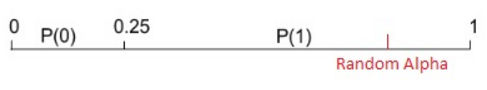
\includegraphics[angle=0,width=0.5\textwidth]{paq.png}
		\caption{Example of sampling}
		\label{fig1}
	\end{center}
\end{figure}

It was noted that granting too much freedom to the compressor could result in a large accumulation of bad predictions, leading to poor text generation. Therefore, it is proposed to make the text generation more conservative adding a parameter called "temperature" that reduces the possible range of the random number as shown in Figure \ref{fig2}.

On maximum temperature, the random number will be generated in the interval [0,1), giving the compressor maximum degree of freedom to make mistakes, whereas, when the temperature parameter turns minimum, the "random" number will always be 0.5, removing the degree of freedom to commit errors (in this scenario, the highest probability symbol will be generated). 
\begin{figure}[ht]
	\begin{center}
		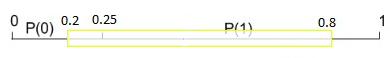
\includegraphics[angle=0,width=0.5\textwidth]{paq2.png}
		\caption{The range is reduced to [0.2, 0.8) when the temperature parameter turns 0.6.}
		\label{fig2}
	\end{center}
\end{figure}

When temperature is around 0.5, the result seems to be actually legible, even if it is not similar to the original text (according to the proposed metrics). This effect is shown at the following randomly generated Harry Potter's snippet:
\newline
\begin{displayquote}
	\textit{``What happened?''  said Harry, and she was standing at him.  ``He is short, and continued to take the shallows, and the three before he did something to happen again.  Harry could hear him.  He was shaking his head, and then to the castle, and the golden thread broke; he should have been a back at him, and the common room, and as he should have to the good one that had been conjured her that the top of his wand too before he said and the looking at him, and he was shaking his head and the many of the giants who would be hot and leafy, its flower beds turned into the song.}
	\newline
\end{displayquote}

\subsection{Metrics}

A simple transformation is applied to each text in order to compute metrics. It consists in counting the number of occurrences of each n-gram in the input (i.e. every time a n-gram "WXY..AZ" is detected, it increases its number of occurrences). 
Then three different metrics were considered:

\subsubsection{Pearson's Chi-Squared}

How likely it is that any observed difference between the sets arose by chance. 
The chi-square is computed as:

$$
\mathcal{X}^2 = \sum_{i=1}^{n} \frac{(O_i - E_i)^2}{E_i}
$$

Where $O_i$ is the observed ith value and $E_i$ is the expected ith value. A value of 0 means equality. This metric is computed using 4-grams.

\subsubsection{Total Variation}

Each n-gram's observed frequency can be denoted like a probability if it is divided by the sum of all frequencies, P(i) on the real text and Q(i) on the generated one. 
Total variation distance \cite{Variation} can be computed according to the following formula:

$$
\delta(P,Q) = \frac{1}{2} \sum_{i=1}^{n} |P_i - Q_i| 
$$

In other words, the total variation distance is the largest possible difference between the probabilities that two probability distributions can assign to the same event. A value of 0 means equality. This metric is computed using 4-grams.

\subsubsection{Generalized Jaccard Similarity}

It is the size of the intersection divided by the size of the union of the sample sets \cite{Chierichetti}. Jaccard Similarity is computed using the following formula:

$$
J(G,T) = \frac{G \cap T}{G \cup T}
$$

Given two non-negative n-dimensional real vectors X, Y , their Jaccard similarity is defined as \cite{Chierichetti}:

$$
J(x,y) = \frac{\sum_{i=1}^{n} min(X_i , Y_i)}{\sum_{i=1}^{n} max(X_i , Y_i)}
$$
This last definition is also know as "Weighted Jaccard Similarity". A value of 1 means both texts are equals. This metric is computed using 10-grams.

\subsection{About Samples}
For each scenario, the RNN was trained several times to find its best hyper-parameters. Asymmetrically, the compressor required to be trained just once. After that, a sampling procedure was executed. It set up different values for "temperature" parameter, allowing these trained models to generate diverse text samples It must be noticed that very high temperatures produce text that is not so similar to the training test, temperatures that are too low aren't also optimal, the best value is usually an intermediate one as shown in Figure \ref{fig3}.

\begin{figure}[hb]
	\begin{center}
		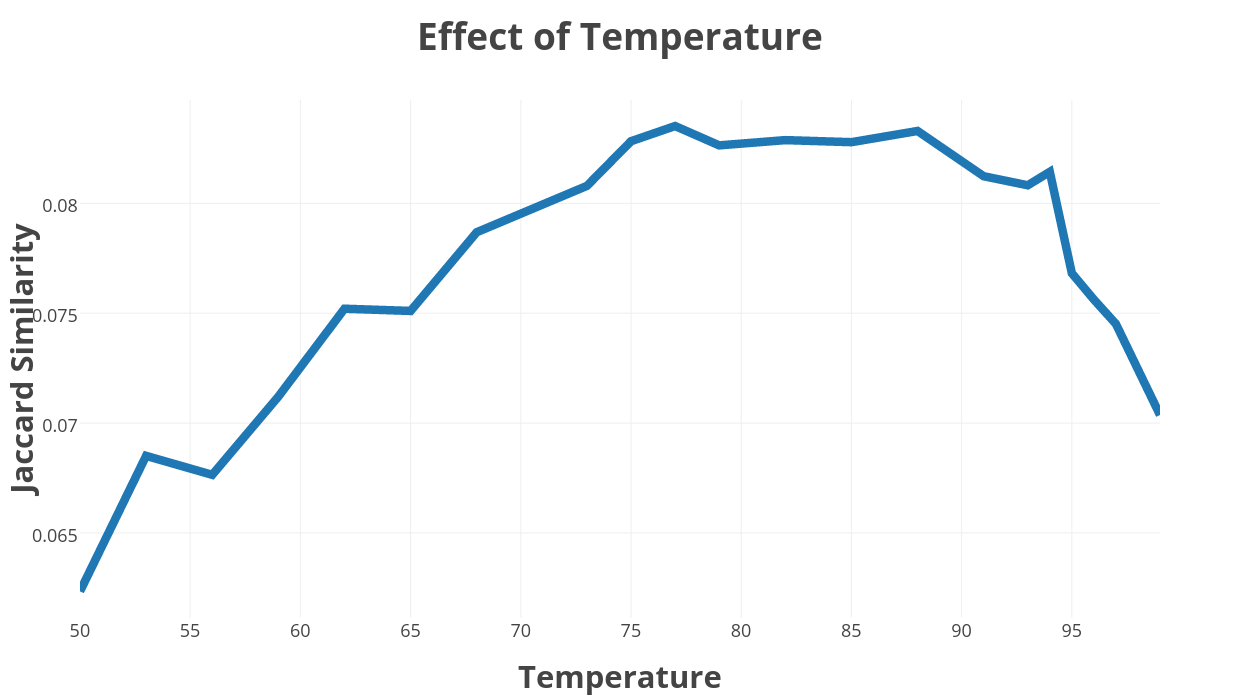
\includegraphics[angle=0,width=0.5\textwidth]{temp.png}
		\caption{Effect of Temperature in the Jaccard Similarity}
		\label{fig3}
	\end{center}
\end{figure}

In this research, similarity between the input text (e.g. The Complete Works of William Shakespeare) and an automatic generated text sample was measured using a local context and a global one. 
\begin{enumerate}
	\item Local similarity: The input text is splitted into $n$ fragments. Then, the metric is computed using each fragment against the generated text. Given the fact that this technique produces $n$ values, the best value is taken.
	\item Global similarity: The metric is computed using the input text against the generated one. There is no fragmentation.
\end{enumerate}

\subsection{Results}
Turning off the training process and the weights adjustment of each model freezes the compressor's global context at the end of the training set. As a consequence of this event, the last piece of the entry text will be considered as a "big seed".

For example, The King James Version of the Holy Bible includes an index at the end of the text, a bad seed for text generation. Compressing the Bible with that index set an unknown context for PAQ and leaded us to this result:
\newline
\begin{displayquote}
	\textit{\^{}55And if meat is
		broken behold I will love for the foresaid shall appear, and heard
		anguish, and height coming in the face as a brightness is for God shall
		give thee angels to come fruit.
		\newline
		\newline
		56But whoso shall admonish them were dim born also for the gift
		before God out the least was in the Spirit into the company
		\newline
		\newline
		[67Blessed shall be loosed in heaven.)}
	\newline 
\end{displayquote}

The index at the end of the file was removed and then PAQ compressed and generated again:
\newline
\begin{displayquote}
	\textit{\^{}12The flesh which worship him, he of our Lord Jesus Christ be with you
		most holy faith, Lord, Let not the blood of fire burning our habitation
		of merciful, and over the whole of life with mine own righteousness,
		shall increased their goods to forgive us our out of the city in the
		sight of the kings of the wise, and the last, and these in the
		temple of the blind.
		\newline
		\newline
		\^{}13For which the like unto the souls to the saints salvation, I saw in the
		place which when they that be of the bridegroom, and holy partly, and
		as of the temple of men, so we say a shame for a worshipped his face: I
		will come from his place, declaring into the glory to the behold a
		good; and loosed.
		\newline  
		\newline 
		\^{}14He that worketh in us, by the Spirit saith unto the earth;and he
		that they shall not be ashamed before mine old, I come saith unto
		him the second time, and prayed, saying to flower, and death reigned
		brass.}
	\newline 
\end{displayquote}

The difference is remarkable. Comparing different segments of each input file against each other, it was observed that in some files the last piece was significantly different than the rest of the text. Those unpredictable endings mess up PAQ's generation but it was very interesting to notice that for the RNN did not result in a noticeable difference. This was the first hint that the compressor and the RNN were proceeding in different ways. An example of the impact caused by choosing a good seed is given in Figure \ref{fig4}.
\begin{figure}[b]
	\begin{center}
		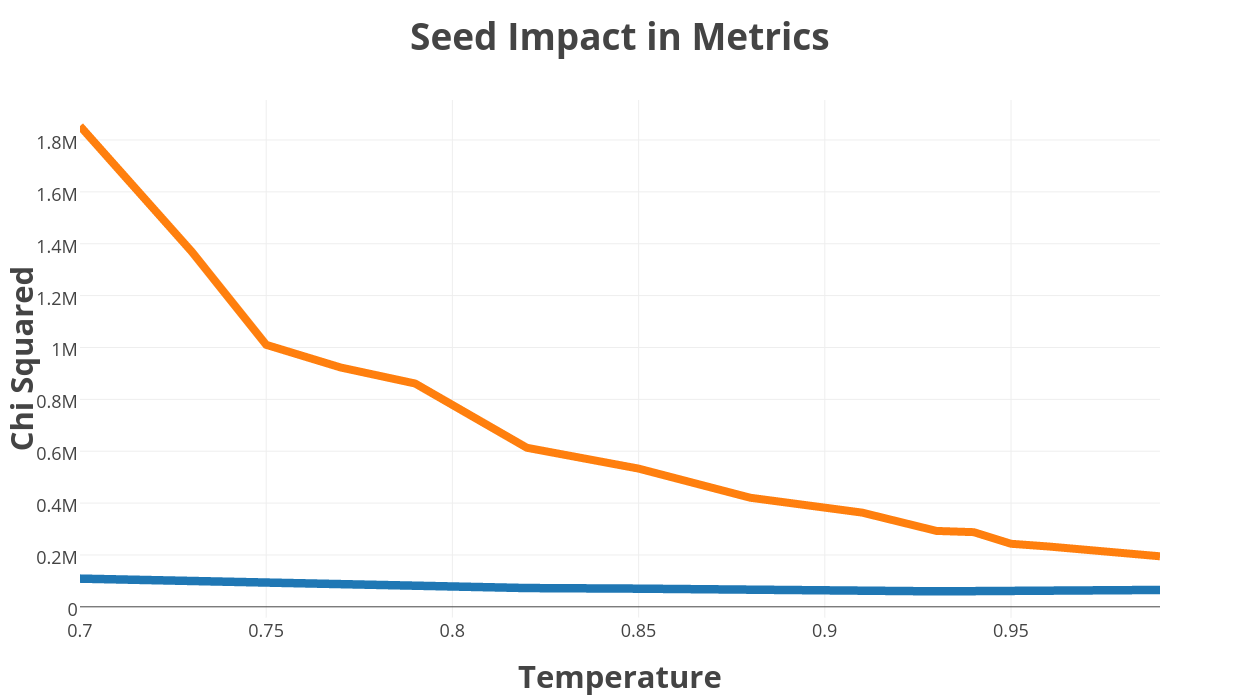
\includegraphics[angle=0,width=0.5\textwidth]{chiseed.png}
		\caption{The effect of a chosen seed in the Chi Squared metric. In Orange the metric variation by temperature using a random seed. In Blue the same metric with a chosen one.}
		\label{fig4}
	\end{center}
\end{figure}
In some cases the compressor generated text that was surprisingly well written. 
\newline
\newline
This is an example of random text generated by PAQ8L after compressing Harry Potter:
\begin{displayquote}
\textit{CHAPTER THIRTY-SEVEN - THE GOBLET OF LORD VOLDEMORT OF THE FIREBOLT MARE!"
	\newline
	\newline
	Harry looked around.  Harry knew exactly who lopsided, looking out parents. They had happened on satin' keep his tables.''
	\newline
	\newline
	Dumbledore stopped their way down in days and after her winged around him.
	\newline
	\newline
	He was like working, his eyes.  He doing you were draped in fear of them to study of your families to kill, that the beetle, he time.  Karkaroff looked like this.  It was less frightening you.}
\newline
\end{displayquote}
Another example, this one was generated after compressing Linux Kernel:
\begin{lstlisting}
#ifdef CONFIG_CONSTRUCTORS

struct inode *inode;
	int setup_init(trace->flags, pause_on_oops)
{
	int smp_mb__after_atomic();
	struct hd_struct *p;
	const char *t;
	int modinfo_next_pid_nr(current));
}
/*
 * Information about the signal context, int that freezers placement states if
 * since periodic);
 */
int cpumask_var_node(&context, unsigned long usermodehelper_execution(struct task_struct *prev)
{
	struct module_attribute *attribute, struct module_kobject *mk;
	int ret;
	bool boolval;
}
\end{lstlisting}
An automatic Game of thrones' snippet:
\begin{displayquote}
\textit{
Page 775
\newline\newline
Summer, or closed with a leather shield, so suddenly. Mero went too. She leaves. There was a fire silver smoke. 
"No one and losing herself and said the maester gorne a moment." 
Ser Robin King Joffrey, though for a bolt of the wind and a sword with your brothers and frozen too far 
and after he was finished the wine and a chainmail. They plotted hands, he had habit for her, slid unknowable,
\newline}
\end{displayquote}

\begin{displayquote}
\textit{
Page 776
\newline\newline
"From is no tears, and began to gather himself that be well sited and a watch benches can't say, mercy 
for him to her here. They say me have made more distinct that after another, and seized her. One was 
many too. His neck and danced into the solar, like the other. He staggered him and something else the sky began, the blankets. The walls 
son was dry jests. Lord Mormont feebly. I am many horses. Not only was not sorry he had no heed her a 
moment. I saw his castle, but he thought of his personal emblem. He might have been long and the hall grey 
mantle opened the outer was never been so heavily he saw no sign of Craven she said of a shadowcat and her smiled 
looked candle had deflowered, a chunk of bread. "And count. It's not here, eating was a handsome unscathed.}
\end{displayquote}

While the text may not make sense it certainly follows the style, syntax and writing conventions of the training text.

\subsection{Metric Results}


In this section, the results of both algorithms are shown so that to evaluate how much similar the results are to the original inputs.

\subsubsection{Local similarity}


Tables \ref{tab:localchi}, \ref{tab:localtotal} and \ref{tab:localjaccard} show local similarity results. It can be seen that the compressor got better results for all texts except Poe, Shakespeare and Game of Thrones. A subtle reason why the RNN got better results in such texts is explained in the conclusions.

\begin{table}[!hbt]
	\begin{center}
		{\caption{Chi Squared Results (Local similarity).}\label{tab:localchi}}
		\begin{tabular}{|l|l|l|}\hline
			&\textbf{PAQ8L} & \textbf{RNN}\\ \hline
			Game of Thrones & 47790 & \textbf{44935} \\ 
			Harry Potter & \textbf{46195} & 83011 \\
			Paulo Coelho & \textbf{45821} & 86854 \\
			Bible & \textbf{47833} & 52898 \\
			Poe & 	61945 & \textbf{57022} \\
			Shakespeare & \textbf{60585} & 84858 \\
			Math Collection & \textbf{84758} & 135798 \\
			War and Peace & \textbf{46699} & 47590 \\
			Linux Kernel & \textbf{136058} & 175293 \\ \hline
		\end{tabular}
	\end{center}
\end{table}

\begin{table}[!hbt]
	\begin{center}
		{\caption{Total Variation \%(Local similarity).}\label{tab:localtotal}}
		\begin{tabular}{|l|l|l|}\hline
			&\textbf{PAQ8L} & \textbf{RNN}\\ \hline
			Game of Thrones & 25.21 & \textbf{24.59} \\
			Harry Potter & \textbf{25.58} & 37.40 \\
			Paulo Coelho & \textbf{25.15} & 34.80 \\
			Bible &  \textbf{25.15} & 25.88 \\
			Poe & 30.23 & \textbf{27.88} \\
			Shakespeare & \textbf{27.94} & 30.71\\
			Math Collection & \textbf{31.05} & 35.85 \\
			War and Peace & \textbf{24.63} & 25.07 \\
			Linux Kernel & \textbf{44.74} & 45.22 \\ \hline
		\end{tabular}
	\end{center}
\end{table}

\begin{table}[!hbt]
	\begin{center}
		{\caption{Jaccard Similarity (Local similarity).}\label{tab:localjaccard}}
		\begin{tabular}{|l|l|l|}\hline
			&\textbf{PAQ8L} & \textbf{RNN}\\ \hline
			Game of Thrones & 0.06118 & \textbf{0.0638} \\
			Harry Potter &  \textbf{0.1095} & 0.0387 \\f
			Paulo Coelho &  \textbf{0.0825} & 0.0367 \\
			Bible &  \textbf{0.1419} & 0.1310 \\
			Poe & 	0.0602 & \textbf{0.0605} \\
			Shakespeare & 0.0333 & \textbf{0.04016} \\
			Math Collection & \textbf{0.21} & 0.1626 \\
			War and Peace & \textbf{0.0753} & 0.0689 \\
			Linux Kernel & \textbf{0.0738} & 0.0713 \\ \hline
		\end{tabular}
	\end{center}
\end{table}

\subsubsection{Global similarity}
The Recurrent Neural Network got better results in global contexts. The results are shown in Tables \ref{tab:globalchi}, \ref{tab:globaltotal} and \ref{tab:globaljaccard}

\begin{table}[!hbt]
	\begin{center}
		{\caption{Chi Squared Results (Global similarity).}\label{tab:globalchi}}
		\begin{tabular}{|l|l|l|}\hline
			&\textbf{PAQ8L} & \textbf{RNN}\\ \hline
			Game of Thrones & \textbf{60541} & 62514 \\ 
			Harry Potter & \textbf{66008} & 363711 \\
			Paulo Coelho & \textbf{67846} & 255951 \\
			Bible & 838686 & \textbf{70258} \\
			Poe & 	99199 & \textbf{75965} \\
			Shakespeare & 180619 & \textbf{91877} \\
			Math Collection & 294999 & \textbf{100153} \\
			War and Peace & \textbf{59625} & 62854 \\
			Linux Kernel & 371226 & \textbf{198317} \\ \hline
		\end{tabular}
	\end{center}
\end{table}

\begin{table}[!hbt]
	\begin{center}
		{\caption{Total Variation \%(Global similarity).}\label{tab:globaltotal}}
		\begin{tabular}{|l|l|l|}\hline
			&\textbf{PAQ8L} & \textbf{RNN}\\ \hline
			Game of Thrones & 21.79 & \textbf{19.16} \\
			Harry Potter & \textbf{25.31} & 33.67 \\
			Paulo Coelho & \textbf{24.92} & 30.62 \\
			Bible &  28.51 & \textbf{17.21} \\
			Poe & 29.63 & \textbf{21.39} \\
			Shakespeare & 29.63 & \textbf{21.67}\\
			Math Collection & 36.46 & \textbf{22.78} \\
			War and Peace & 37.38 & \textbf{18.81} \\
			Linux Kernel & 41.85 & \textbf{29.70} \\ \hline
		\end{tabular}
	\end{center}
\end{table}

\begin{table}[!hbt]
	\begin{center}
		{\caption{Jaccard Similarity (Global similarity).}\label{tab:globaljaccard}}
		\begin{tabular}{|l|l|l|}\hline
			&\textbf{PAQ8L} & \textbf{RNN}\\ \hline
			Game of Thrones & 0.0611 & \textbf{0.0636} \\
			Harry Potter &  \textbf{0.0835} & 0.0386 \\
			Paulo Coelho &  \textbf{0.0758} & 0.0399 \\
			Bible &  0.0911 & \textbf{0.1430} \\
			Poe & 	0.0500 & \textbf{0.0646} \\
			Shakespeare & 0.0332 & \textbf{0.0401} \\
			Math Collection & 0.1351 & \textbf{0.2094} \\
			War and Peace & 0.0427 & \textbf{0.0761} \\
			Linux Kernel & 0.0771 & \textbf{0.0925} \\ \hline
		\end{tabular}
	\end{center}
\end{table}

\section{Conclusions}

In the sentiment analysis task, an improvement using PAQ over a Neural Network is noticed. A Data Compression algorithm has the intelligence to understand text up to the point of being able to predict its sentiment with similar or better results than the state of the art in sentiment analysis. In some cases the precision improvement was up to 6\% which is a lot. 

Sentiment analysis is a predictive task, the goal is to predict sentiment based on previously seen samples for both positive and negative sentiment, in this regard a compression algorithm seems to be a better predictor than a RNN.

In the text generation task, the use of a right seed is needed for PAQ algorithm to be able to generate useful text, this was evident in the Bible example. This result is consistent with the sentiment analysis result because the seed is acting like the previously seen reviews, if it is not in sync with the text then the results will not be similar to the original text.

The text generation task showed the critical difference between a Data Compression algorithm and a Recurrent Neural Network and according to our research this is the most important result: Data Compression algorithms are \textit{predictors} while Recurrent Neural Networks are \textit{imitators}.

The text generated by a RNN looks in general better than the text generated by a Data Compressor but if just one paragraph is generated, the Data Compressor is clearly better. PAQ learns from the previously seen text and creates a model that is optimal for predicting what is next, that is why they work so well for Data Compression and that is why they are also very good for Sentiment Analysis or to create a paragraph after seeing the training set. 

On the other hand the RNN is a great imitator of what it learned, it can replicate style, syntax and other writing conventions with a surprising level of detail but what the RNN generates is based on the whole text used for training without weighting recent text as more relevant. In this sense, the RNN is better for random text generation while the Compression algorithm should be better for random text extension or completion.

Suppose the text of Romeo \& Juliet is located at the end of William Shakespeare's works and then both algorithms use them to generate a sample. As a consequence, PAQ would create a new paragraph of Romeo and Juliet whereas the RNN would generate a Shakespeare-like piece of text. \textbf{Data Compressors are better for local predictions and RNNs are better for global predictions.}

This explains why in the text generation process PAQ and the RNN obtained different results for different training tests. PAQ struggled with "Poe" or "Game of Thrones" but was very good with "Coelho" or the Linux Kernel. What really happened was that it was measured how predictable the last piece of the text was!. If the text is very predictable then the best predictor will win, PAQ defeated the RNN by a margin with the Linux Kernel and Paulo Coelho. When the text is not predictable then the ability to imitate in the RNN defeated PAQ. This can be used as a wonderful tool to evaluate the predictability of different authors comparing if the Compressor or the RNN works better to generate similar text. In our experiment it was concluded that Coelho is more Predictable than Poe and it makes all the sense in the world!

As our final conclusion it was shown that Data Compression algorithms show rational behaviour and that they are based on the accurate prediction of what will follow, based on what they have learnt recently. RNNs learn a global model from the training data and can then replicate it. That is why Data Compression algorithms are great \textbf{predictors} while Recurrent Neural Networks are great \textbf{imitators}. Depending on which ability is needed one or the other may provide the better results. 

\section{Future Work}

From our point of view, Data Compression algorithms could be used with a certain degree of optimality for any Natural Language Processing Task where predictions are made with the recent local context. Completion of text, seed based text generation, sentiment analysis, text clustering are some of the areas where Compressors might play a significant role in the near future.

We have also shown that the difference between a Compressor and a RNN can be used as a way to evaluate the predictability of the writing style of a given text. This might be expended in algorithms that can analyze the level of creativity in text and can be applied to books or movie scripts.

\section*{Acknowledgements}
This research was supported by Universidad de Buenos Aires. We thank our colleagues who provided insight and expertise that greatly assisted the research.
\newline
\newline
We thank researchers from Argentine Symposium of Artificial Intelligence for comments that greatly improved the manuscript. 
\newline
\newline
We would also like to show our gratitude to Dr. Matt Mahoney for sharing his knowledge in compression algorithms. We are also immensely grateful to Dr. Alex Graves for his comments on an earlier attempt to make handwriting recognition with PAQ compressor

\nocite{*}
\bibliographystyle{plain}
\bibliography{References}

\end{document}
